\documentclass{article}
\usepackage[UTF8]{ctex}


\usepackage{amsfonts,amssymb,amsmath}
\usepackage{graphicx}
\usepackage{cite}
\usepackage{paralist}

\newcommand{\jMAVSim}{\textsf{jMAVSim}}

\newcommand{\naturals}{\mathbb{N}}
\newcommand{\reals}{\mathbb{R}}

\newcommand{\expectation}{\mathbb{E}}

\newcommand{\states}{S}
\newcommand{\actions}{A}
\newcommand{\observables}{O}
\newcommand{\trans}{T}
\newcommand{\obs}{Z}
\newcommand{\reward}{R}
\newcommand{\discount}{\gamma}

\newcommand{\beliefs}{\mathcal{B}}
\newcommand{\beliefUpdate}{\tau}

\newcommand{\policy}{\pi}

\newcommand{\diff}[1]{\mathop{}\!\mathrm{d}#1}

\usepackage{hyperref}

\setlength{\tabcolsep}{5pt}
% \allowdisplaybreaks
\title{无人机防碰撞系统的建模和实现}
\author{XXXX}
\begin{document}
\maketitle
\begin{abstract}
随着民用航空领域无人机的应用越来越广泛,无人机的防碰撞系统就显得更加重要和有价值。理想的无人机防碰撞系统会检测到周围无人机的位置,并且根据无人机的位置来选择能够减小碰撞风险的最优的飞行动作。目前在生成防碰撞的策略时,一般使用部分可观测的马尔科夫决策过程(POMDP)对无人机的行为进行建模,并在该模型的基础上进行最优策略的生成。目前已有的防碰撞系统需要敌机的精确位置信息来生成防碰撞的行为,并且忽视飞行路径变化,这样就会出现防碰撞系统的鲁棒性不高,并且计算过程消耗过多的飞行资源的问题。本文根据原始的飞行路径中的有限的信息构建了一个防碰撞系统。我们使用POMDP来进行防碰撞系统的建模,系统仅包含无人机的目标位置信息以及敌机位置变化的模糊信息,并且利用这些信息来生成防碰撞的逻辑。我们实现了一个防碰撞的模块,并将该模块集成到了PX4飞行控制平台上,进行了飞行模拟实验来验证了我们实现的系统的有效性。
\end{abstract}


\section{引言}

安全性对于航空领域至关重要。为了提升安全性,现代的飞行控制包括多个部分,其中包含有对应飞机驾驶资质的良好受训的飞行员,根据飞行状况和地面信号通知飞行员进行飞行行为的空中交通控制系统,以及飞机配备的飞行控制辅助系统。在飞行中最严重的情况就是飞机出现空中的碰撞。通常防止飞机之间相撞的方法可能是通过交通管制系统给出飞机的飞行指令,飞行员按照指令进行飞机操纵,改变航线和高度,在跨洋航行时,飞行员会用机载自动驾驶系统进行辅助飞行。

\subsection{机载防碰撞系统}
随着空中交通的普及,发生空中飞机碰撞的风险也相应的增加了,因此机载防碰撞系统的研发备受航空界关注。在上个世纪60年代到70年代,多个飞机制造商开发了飞机的防碰撞系统,例如BCAS信标防碰撞系统。BCAS通过接收地面的信标防碰撞系统发来的信号数据来确定敌机的距离和高度。1978年,美国联邦航空局开始开发交通预警防碰撞系统TCAS\cite{9,10},该系统现今被广泛应用于航空领域。TCAS是对BCAS的改进版本,TCAS不仅能够获得敌机的位置信息,还能根据这些信息给出飞机操控行为的建议,例如给出应该改变爬升率和下降率给飞行员,从而减少碰撞的风险。经过几十年的对防碰撞系统的开发与改进,TCAS目前是大型客运以及货运机型上的必备系统。
TCAS使用一个机载的信标雷达来监控空中的交通状态并通过防碰撞的逻辑对可能接近的空中碰撞风险给出飞行员相关的预警信号以及操作建议。 TCAS防碰撞逻辑是根据飞行控制的几十年的经验来构建的,在实现之初,就已经通过了模拟的检验并保证了飞行控制系统的安全性和操作上的可接受性。但是基于经验构建的防碰撞系统在鲁棒性上可能就存在不足。比如该系统不会考虑如果飞行员不按照防碰撞系统的指令进行操作时的情况,并且TCAS代码实现较为复杂,完全理解TCAS的整个控制逻辑比较困难,更不用说对逻辑进行修改。文献\cite{9}中就给出了TCAS相关的开发,并且介绍了机防碰撞系统的相关细节。

\subsection{无人机防碰撞系统的进展}
近些年,随着无人机的不断发展和应用,许多研究开始对无人机的防碰撞进行探讨并开发无人机的防碰撞系统。其中比较有名的是ACAS X机载防碰撞系统\cite{8}。ACAS X当前将飞机附近的飞行环境用一个部分可观测的马尔科夫决策过程来进行建模,并却用动态规划算法来计算POMDP的最优策略,来尽可能的减少碰撞发生的可能性。在计算出最优策略后,防碰撞系统将策略存储在表中,飞行器可以根据当前的状态和表,查到当前应该采取的最优的行动,以最大程度地避免碰撞的发生。在\cite{8}中,ACAS X生成的防碰撞处理逻辑在鲁棒性、效率以及灵活性等层面上都超过超过了之前使用的TCAS系统。
ACAS Xu,是ACAS X系统针对于无人机的版本,其中u表示无人机,该系统目前仍在研发中。实际上,无人机的利用和普及使得目前无论是无人还是有人操纵的飞行器,都需要考虑无人机和一般飞机的飞行行为。无人机在以下场景中有着丰富的应用,无人机在军事应用领域已经开始显得愈发重要,由于无人机的轻量化、良好的隐蔽性以及对于飞行人员来说的安全性,受到军事应用的青睐。军用无人机在集群作战、设备运输以及设施保护等多个方面都有这越来越重要的作用。在民用航空领域,无人机在航空影像、快递运输等方面也扮演重要角色。公共领域无人飞行器的普及,对无人航空器的安全性就有着更高的要求,特别是对于空中防碰撞的要求,这需要无人机有着在空中感知其他飞行单位,并根据其他飞行单位的位置作出防碰撞飞行动作的能力。
和一般的民航客机和货机相比,无人机的防碰撞系统面临着更多的挑战,比如无人机有着更复杂的飞行环境,更弱的环境感知能力以及更短的防碰撞动作触发时间,这些都使得保证无人机防碰撞系统的正确性变得更加困难。和大型固定翼客运和货运飞机相比\cite{12},无人机的防碰撞有着以下的难点:(1)无人机需要使用更便宜、轻量化以及抗噪能力更强的传感器。(2)固定翼飞机的飞行行为有着固定的动作控制,而无人机的飞行行为更加复杂。(3)ACAS X仅仅提供垂直方向的控制,而无人机在水平方向和垂直方向上都有防碰撞的要求。
在无人机防碰撞领域已经有许多相关的研究\cite{1,5,20}。在\cite{20}中,该文章用POMDP来对只能对环境有有限的观测能力的防碰撞系统进行建模,并在离散的状态空间中利用迭代算法计算出策略,并且在全球鹰无人机模拟器上进行了实验验证\cite{1}。\cite{1}直接解决了连续状态空间中的POMDP来解决高维空间中的状态空间的请哭那个。\cite{5}利用深度神经网络来学习一个近似的查找表,但是他们和我们的工作的差距在于,他们没有在真实的系统上来实现这个防碰撞的逻辑,并且他们的仿真并没有考虑过多的飞行动作会对飞机本身的飞行轨迹产生影响,在我们的工作中我们考虑了这一点。
以上所提到的工作一般更加依赖于从传感器获得的敌机的精确位置信息(比如位置、与本机距离等)来生成防碰撞的行为。在实际情况下,由于传感器的能力限制,我们并不能获得如此详尽的敌机和当前飞机的信息,因此要么这些防碰撞系统的鲁棒性不高,要么获得精确信息占用了太多的无人机的计算资源,对计算资源造成了浪费。

\subsection{本文的贡献}

为了解决以上提出的问题,本文提出了针对于仅能获得敌机有限信息的防碰撞系统,并且该防碰撞系统能尽量简化对于无人机的操作,以减小对无人机原有的飞行行为的变化,以节省飞行资源。我们仍然用POMDP来对只有目的地信息,敌机和本机的粗略飞行信息的防碰撞系统进行建模,并利用该POMDP模型来生成防碰撞逻辑。通过在Pixhawk模拟器上进行了模拟实验,并且我们还将该防碰撞模块集成到了Pixhawk无人机系统上,并将防碰撞模块的实现集成到了真实的飞行控制平台PX4上,能够在真实环境中进行飞行。从本文在Pixhawk无人机平台上的实验可以看出,我们生成的防碰撞逻辑在真实飞行情况下也有着不错的表现。



\section{部分可观测马尔科夫决策过程}
这一节主要回顾POMDP的相关定义以及\cite{1}中如何给出的无人机防碰撞的解决方案。

对于一个在随机环境下的智能体(例如本文无人机碰撞系统中的无人机)。该智能体和环境一同构成了我们研究的整个系统,该系统会记录智能体和环境所在的状态。在每个单位时间内,智能体通过观察整个系统所处的状态,来决定下一步需要执行的动作,该动作又会产生智能体本身的状态变化,从而影响到整个系统的状态。在概率模型中,我们通常使用一个状态的概率分布,来表示智能体在执行一个动作后的结果的不确定性。当系统的状态空间对智能体完全可知的时候,我们可以用马尔科夫决策过程(MDP)直接对系统建模\cite{15}。但如果只能提仅仅知道系统状态的部分信息时,用部分可观测马尔科夫决策过程就能更好的对这样的情况进行建模。在无人机这个场景下,部分可观测具体可能是无人机配备了带有噪音的传感器,不能获得或者不能区分获得的数据是否精确,也就不能确定敌机的精确的位置信息,而是仅能知道一个粗糙的对于位置信息的描述(例如敌机在左侧、右侧等)。

POMDP对MDP模型进行扩展,POMDP隐藏了MDP中可见的当前所在的实际状态,并提供了一个观测进程根据当前所在的状态随机的生成观测。POMDP对智能体的决策过程进行建模,智能体决策过程通过对系统的回报值的相关分析和计算,能够得到一个使得总回报值最大的动作序列。但是这个过程中,智能体并不能精确的知道系统的所在的状态,而是只能得到状态的观测。不同的系统可能得到的观测是相同的。智能体会用一个状态的概率分布来表示其对于当前所在状态的信念,并会根据采取的不同动作以及得到的观测来改变信念。

\subsection{POMDP具体定义}


一个部分可观测的马尔科夫决策过程是一个七元组$(\states, \actions, \observables, \trans, \obs, \reward, \discount)$,其中$\states$, $\actions$, $\observables$分别表示状态、动作以及系统的观测空间。$\trans \colon \states \times \actions \times \states \to [0,1]$ 和 $\obs \colon \states \times \actions \times \observables \to [0,1]$分别是迁移函数以及观测函数。对于每个状态 $s \in \states$和动作 $a \in \actions$, 以及迁移后的状态$s' \in \states$ 和观测 $o \in \observables$, 对迁移函数以及观测函数我们有$\trans(s, a, s') = p_{\states}(s' | s, a)$ 以及 $\obs(s, a, o) = p_{\observables}(o | s, a)$。其中概率分布 $p_{\states}$ 和 $p_{\observables}$ 分别用来对系统动力学和观测建模;$\reward \colon \states \times \actions \to \reals$ 是回报函数;
$\discount \in [0,1)$ 是用来平衡即期回报和远期回报的折扣因子。 在这篇文章中,我们假设动作集合 $\actions$ 和观测集合 $\observables$ 都是有穷的。

POMDP在每个状态的每一步都按照下面的方式进行执行:当系统在状态$s \in \states$执行动作$a \in \actions$时,系统会进行以下行为:
\begin{inparaenum}[1)]
\item
	获得在状态$s$执行动作$a$的回报值$r = \reward(s,a)$;
\item
	系统迁移到以概率$\trans(s, a, s')$迁移到状态$s'$;
\item
	以$\obs(s', a, o)$的概率在 $s'$产生一个观测$o \in \observables$。
\end{inparaenum}
这里需要注意观测依赖于迁移之后的具体状态。

由于智能体仅对当前系统处在的状态保存一个信念,因此在执行动作$a$并获得观测$o$来对当前的信念做改变。我们令$\beliefs$表示信念的集合,也就是状态上的概率分布的集合。给定一个信念 $b \in \beliefs$, 在执行动作$a$ 并得到观测 $o$之后, 智能体通过以下公式来更新对于迁移到的$s'$的信念:
\begin{equation} 
	b^{o}_{a}(s') = \eta \obs(s', a, o) \int_{s \in \states} \trans(s, a, s')  b(s) \diff{s},
	\label{eq:beliefUpdate}
\end{equation}
其中 $\eta$是一个使得积分$\int_{s \in \states} b^{o}_{a}(s) = 1$的正规化因子。为了简化标记,当$a$ 和$o$都清晰的时候,我们$b'$ 来表示 $b^{o}_{a}$。更新信念的过程在是贝叶斯规则的直接应用,也叫状态估计或者过滤~\cite{book}.

\subsection{POMDP 模型与求解}

POMDP和MDP类似,都有不确定性以及概率的行为。不确定性体现在,对于一个状态可以执行的不同的动作,我们是通过智能体的策略 $\policy$ 来表示在每个状态智能体的行为选择, 也就是说策略是一个根据当前对于状态的信念到执行动作的一个映射,可以表示为$\policy \colon \beliefs \to \actions$.

智能体的执行过程可以看作一个动作选择和信念更新两个操作交织的一个序列。给定一个策略$\policy$以及当前智能体的信念$b$,智能体的控制系统通过策略计算出当前的动作$a = \policy(b)$. 然后在执行完动作后,又会根据公式~\ref{eq:beliefUpdate}中更新信念的公式来进行更新。

求解POMDP的最优策略$\policy^{*}$的目标就是最大化智能体的平均总体回报,可以用 $\expectation(\sum_{n=0}^{\infty} \discount^{n} \reward(s_{n}, a_{n}))$来表示,其中$s_n$和$a_n$表示系统在第$n$步的状态以及选取的动作。给定一个策略$\policy$我们可以给出该策略的值函数$V_{\policy} \colon \beliefs \to \reals$来表示期望全体回报。策略$\policy$的全体回报的值可以根据以下公式给出:
\begin{equation}
	V_{\policy}(b) = \expectation\big(\sum_{n=0}^{\infty} \discount^{n} \reward(s_{n}, a_{n}) | \policy, b\big).
\end{equation}

在实现层面上,即使是对于例如\cite{ASurveyofPBPOMDP}中的小规模的问题,求POMDP的最优策略这一问题的计算复杂性很高。精确求解最有策略的相关算法可以在一些文献中找到,比如~\cite{article1}中的witness算法。但是这些精确的求解方法对于大规模的例子在实际计算上并不可行。为了使得在大规模的POMDP模型上,其最优策略也能够被求解,常见的方式是考虑求最有策略的近似解,例如在\cite{article2}中所提到的近似求解算法。其中比较成功的算法是基于点的POMDP算法,既能支持计算最优策略的近似解,又能应用到大规模的离散系统上\cite{ASurveyofPBPOMDP,PBVI}。
由于最优值函数 $V^{*}$ 满足以下Bellman方程\cite{article3}
\begin{equation}
	\begin{aligned}
		V^{*}(b) & = H(V^{*}(b)) \\
		& = \max_{a \in \actions} \Big\{\int_{s \in \states} \reward(s,a) b(s) \diff{s} + \discount \sum_{o \in \observables} p(o | b, a) V^{*}(b^{o}_{a})\Big\}
	\end{aligned}
	\label{eq:bellman}
\end{equation}
其中$H$称为\emph{backup} 算子, 大多数计算方法都用它来计算最优值 $V^{*}$. 值迭代算法是基于Bellman方程解MDP最优策略的常见的动态规划算法\cite{RLIntro},在POMDP的算法中,我们也用到值迭代算法的相关结构\cite{ASurveyofPBPOMDP}。

在值迭代的过程中,首先通过已知初始值的相关信息给出的值函数 $V$。
如果一开始我们不知道任何信息,那么对于所有的信念 $V$ 会被设为 $0$。
然后算法会在 $V$上不断的迭代用$H$  计算Bellman方程直到到一个不动点。
当迭代过程终止时,计算出来的策略就是对于每个信念$b$都满足Bellman方程的动作$a$. 

在实现这个算法时,如果直接实现,值迭代算法需要对整个信念空间$\beliefs$进行搜索,在现实问题下就会遇到为多以及指数复杂度的问题。~\cite{ASurveyofPBPOMDP}. 
两个基于点的算法在提高计算效率上起了至关重要的作用。~\cite{MCVI}. 
首先是用从信念空间 $\beliefs$ 上随机采样得到的点作为信念空间的 $\beliefs$的近似表示. 
算法的backup操作是在信念空间的采样点上去计算而不是整个信念空间,因此计算出来的最有策略是一个近似最优策略。
其次,$\alpha$-向量~\cite{sarsop} 被用来作为值函数的近似 $V_{\policy} \colon \beliefs \to \reals$ 来表示从信念$b$开始的执行策略$\policy$的期望总体回报值。
最优值函数可以用形如$
	V^{*}(b) = \max_{\alpha \in \Gamma} \alpha \cdot b
$分段函数和图函数~\cite{Sondik78}来表示
,
其中 $\Gamma = \{\alpha_{0}, \alpha_{1}, \dotsc, \alpha_{m}\}$ 是一个含有  $m$ 个向量,我们把它称作 $\alpha$-向量.
直观上来说, 每个 $\alpha$-向量都能和一个动作相联系。对于当前的信念$b$来说,求解的策略会选在使得 $\alpha$-向量最优的动作。
因此策略同样也可以用含有$\alpha$-向量的$\Gamma$来表示\cite{sarsop}.
通过$\alpha$-向量的方式, 在一定合适的条件下,我们能用目前计算出来的策略为信念空间中剩下的部分计算最优策略,从而显著地提高计算的效率~\cite{ASurveyofPBPOMDP}.

基于点的算法和一般算法的不同在于信念空间上的采样以及执行backup操作的不同。
PBVI~\cite{PBVI} 是第一个在大规模的POMDP上成功应用基于点的算法的样例。
HSVI2~\cite{PBVII} 使用启发式的方法来指导在信念空间上的采样, 这么做可以减少值函数的上界和下届之间的差距,从而达到加速的目的。
SARSOP~\cite{sarsop} 和 HSVI2的方法相关, 但在这篇文章中,作者尝试用增强学习和约束的技术对从初始信念$b_{0}$到最优的可达空间$\mathcal{R}^{*}(b_{0})$进行采样。

尽管基于点的算法在求解离散的POMDP上有着很好的结果, 在连续状态空间的POMDP基于点的算法目前没有太多研究的进展. 
连续的 POMDP 模型对于真实世界的行为有着更强的建模和表示能力,然而唯独问题成为连续POMDP模型的一大障碍。
通常对于连续状态空间POMDP的做法是用各自分割出离散的状态集合$\states$,然后用已有的对于离散POMDP的算法来求解。
这个方法的难点是在分割离散状态时,分割出来的状态空间可能还是太大不符合我们的需求。解决这个问题的一个办法是用一个特殊的参数来表示状态的置信度以及值函数。比如高斯分布的线性组合\cite{pbvic}。另外一个想法是用粒子滤波来表示置信度,比如MC-POMDP\cite{mcpomdp}. 
MCVI (Monte Carlo Value Iteration)~\cite{MCVI} 结合了用粒子滤波表示置信度以及离散的基于点的POMDP的$\alpha$-向量的算法。MCVI用策略图$G$来表示解得的策略\cite{MCVI},其中策略图是一个用编码了最优策略图,在图的每个节点上用动作来做标记,在每条边上用一个观测做标记。置信度并不会显式地存放在这个途中。给定一个置信度$b$,MCVI算法从策略图$G$中,以合适的节点$v$为起始点合成一个策略。策略选择的动作,就是$v$上对应标记的动作,然后智能体根据所选的边$(v,v')$走到下一个状态$v'$并且得到边对应的相应的观测$o$。这个过程会一直重复,直到得到最后的策略。

对于每个策略图$G$上的节点$v$,我们可以定义 $\alpha$-函数$\alpha_{v}$,其中$alpha_v(s)$是从状态$s$开始执行策略$\policy_{G,v}$的期望总体回报:

\begin{equation}
\label{eq:alphaPolicy}
	\alpha_{v}(s) = \expectation\big(\sum_{n=0}^{\infty} \discount^{n} \reward(s_{n}, a_{n}) | \policy_{G,v}, s\big).
\end{equation}
策略$\policy_{G,v}$ 下的置信度$b$的值是根据$G$的$\alpha$-函数如下定义:
\begin{equation}
	V_{G}(b) = \max_{v \in G} \int_{s\in S} \alpha_{v}(s) b(s) \diff{s}.
\end{equation}
策略图是通过近似动态规划技术来构建的,MCVI执行蒙特卡罗模拟来对状态空间和置信度空间进行采样。POMDP的最优值函数 $V^{*}$ 是利用方程\eqref{eq:bellman}中的backup操作在可达的置信度集合中的置信度$b$上多次迭代计算得来的。每次backup操作可以选择一个使得期望即时回报和期望总体回报相加之和在下一个置信度上最大的动作。找到这个动作之后,该动作将被加到策略图中,并且让动作和最优决策距离靠近。可达置信度集合是从整个置信空间中采样得到的对于之心空间的近似表示。MCVI方法在处理连续状态上的积分效果较好,因此在使用MCVI方法时应该避免离散化状态空间从而提高效率。在\cite{MCVI}中有着更详细的描述。


\section{Collision Avoidance Models}
\label{sec:collisionAvoidanceModels}

To the best of our knowledge, the algorithms and models used in the latest versions of ACAS X and ACAS Xu are not publicly accessible.
Therefore, we define our model based on the early published version of ACAS X~\cite{ACASX} and ACAS Xu~\cite{DBLP:conf/rss/Bai-RSS-11}.
In our implementation, the aircraft model is parametric and can be easily modified to fit different types of aircraft.
In this work, we use the parameter values from Pixhawk\footnote{\url{https://pixhawk.org/}} and build the model with PX4\footnote{\url{https://dev.px4.io/master/en/index.html}, PX4 Development Guide.}. 

In our model, we consider a simple encounter situation between two aircraft, our own aircraft and an intruder aircraft.
Our own aircraft has no prior knowledge about the flight path of the intruder aircraft, when an encounter happens.
During this period, our own aircraft can only get information about the intruder aircraft's elevation and bearing by sensors onboard.
The collision avoidance system is responsible to control our own aircraft so to keep a safe distance from the intruder by choosing appropriate actions to avoid collision. 

We will describe the state-transition, observation and reward modeling in our model in detail, similarly to the modeling proposed in~\cite{DBLP:conf/rss/Bai-RSS-11}.


\subsection{State-Transition Modeling}
\label{ssec:stateTransitionModeling}

\begin{figure}[t] 
	\centering
	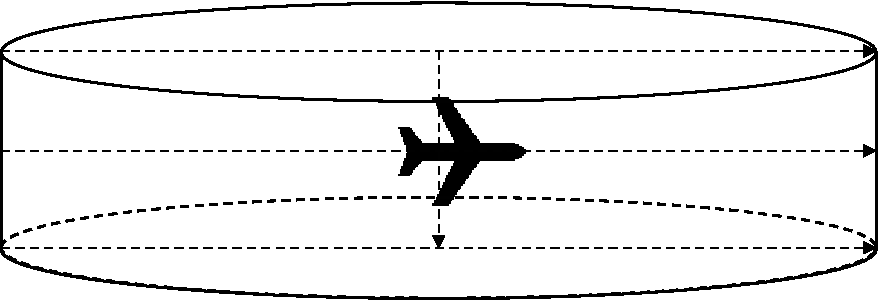
\includegraphics[width=0.40\linewidth]{3dsystem}
	\caption{Threshold range for starting the system in 3D}
	\label{fig:3dsystem}
\end{figure}
The position of a flying aircraft can be represented as a point in the 3-dimensional space.
The collision avoidance system needs to intervene when the horizontal and vertical distances of two aircraft are less than the given thresholds, which depend on the type of the aircraft and other parameters; 
this can be represented as the cylinder shown in Fig.~\ref{fig:3dsystem}.

Similarly to other works on collision avoidance~\cite{25,ACASX}, in order to simplify the model's state space and make verification more practical, we omit the altitude and consider only the latitude/longitude of the aircraft.
So when an intruder is detected, the system tries to avoid the collision by banking left or right, i.e., by changing our aircraft's direction.


\subsubsection{State space.}
Since we ignore the aircraft altitude in our model, we let $(x, y)$ be the position of the aircraft with respect to the Earth coordinate system, where the positive $x$-direction points East and the positive $y$-direction points North.
Let $\theta$ be the heading angle of the aircraft with respect to East and $u$ the aircraft's horizontal forward speed.
The state information of each aircraft is then $(x, y, \theta, u)$.
By combining the information about our aircraft and the intruder, a state in the POMDP representing our model is a $7$-tuple $(x_{1}, y_{1}, \theta_{1}, x_{2}, y_{2}, \theta_{2}, u)$, where $(x_{1}, y_{1}, \theta_{1}, u)$ stands for the state of our own aircraft while $(x_{2}, y_{2}, \theta_{2}, u)$ is the intruder's state, by assuming that both aircraft have the same speed.

The state space of the POMDP is continuous, given the nature of the aircraft information.
In order to compute the next action for our own aircraft, traditional methods have to first discretize the state space by means of a grid, where each grid cell becomes a state of the discrete POMDP~\cite{article}.
In our model, we will directly work in the continuous state space instead.
In this way, we can apply Monte Carlo methods to improve efficiency of the computation of the policy. 

\subsubsection{Action space.}
Now we introduce our modeling of actions.
In order to avoid a collision in an encounter situation, we can change our aircraft direction by changing its forward angle, that is, we bank the aircraft.
Thus we can represent the angular velocity $\omega \in \{-\omega_{m}, 0, \omega_{m}\}$ as an action in our model, where $\omega_{m}$ is the maximum input value for the banking rate.
Consequently, if at step $t$ the heading angle is $\theta_{t}$ and we take the action $\omega$, then the heading angle will become $\theta_{t+1} = \theta_{t} + \omega \Delta t$ at step $t+1 = t + \Delta t$ after a small duration of time $\Delta t$.

\subsubsection{Transition dynamics.}
Now we are ready to give the state-transition dynamics of an aircraft in an encounter situation.
Recall that in our model, a state consists of the information about both aircraft.
Let $s_{t}$ be the state at step $t$ and $s_{t+1}$ the new state at step $t+1$ after a small duration of time $\Delta t$, where $\Delta t$ is the sum of two small durations $\Delta t_{h}$ and $\Delta t_{f}$, i.e., $\Delta t = \Delta t_{h} + \Delta t_{f}$.
In order to avoid a collision, our own aircraft first changes the heading angle by banking $\omega$ degrees for a small amount of time $\Delta t_{h}$ and then goes forward at the constant speed $u$.
After a small amount of time $\Delta t_{u}$, our own aircraft will reach the new position $(x_{t+1}, y_{t+1})$ from $(x_{t},y_{t})$.
This transition dynamics is formalized as follows.
\begin{equation} 
\label{eq:transition}
	\begin{split}
		\theta_{t+1} &= \theta_{t} + \omega \Delta t_{h},\\
		x_{t+1} &= x_{t} + u \Delta t_{f} \cos \theta_{t+1},\\
		y_{t+1} &= y_{t} + u \Delta t_{f} \sin \theta_{t+1}.
	\end{split}
\end{equation}

Note that at the same time, the intruder will also change its flight state $(x_{2}, y_{2}, \theta_{2}, u)$ in a similar way by following the action $\omega_{\mathit{intruder}}$.
Since our own aircraft does not know the action of the intruder, we can model it in different ways:
for instance, the action $\omega_{\mathit{intruder}}$ can be chosen between bank-left, go-forward, and bank-right with equal probability of $\frac{1}{3}$.
Other policies can be used to represent different flight plans for the intruder, such as always banking left or right, to represent an intruder flying in circle;
we can also consider policies where the intruder tries to intercept our aircraft.
We leave the analysis of such policies to the extended version of this paper.



\subsection{Sensor Modeling}
\label{ssec:sensorModeling}

\begin{figure}[t]
	\centering
	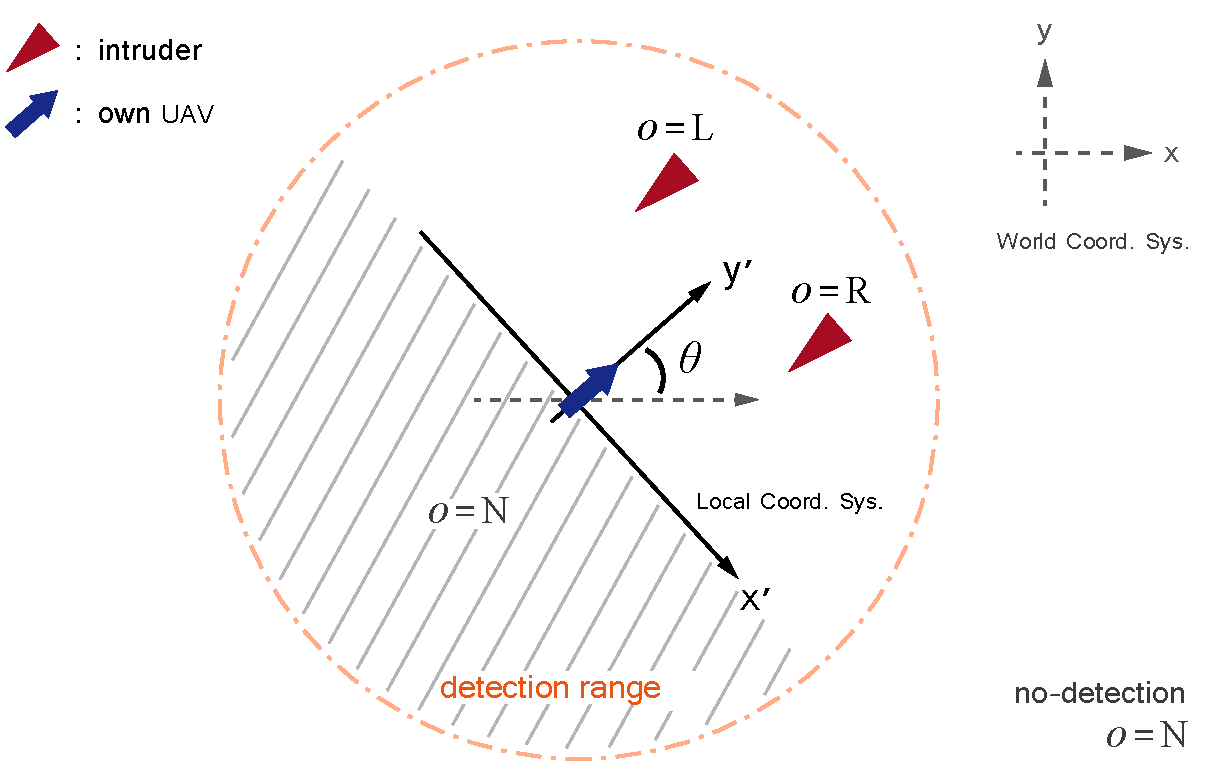
\includegraphics[width=0.7\linewidth]{observationModel}
	\caption{Observation Model}
	\label{fig:observationModel}
\end{figure}
The threat resolution logic behind a collision avoidance system relies on the aircraft on-board sensors to detect intruders.
Electro-optical/infrared (EO/IR) sensors and passive radars are two types of sensors commonly used on large aircraft.
On smaller aircraft, the on-board sensors usually have limited accuracy;
to model this scenario, we use as possible observations $\{N, L, R\}$, which stand for the fact that no intruder is detected, it is detected on the left of the aircraft, or on the right, respectively. 
Fig.~\ref{fig:observationModel} shows the observation values corresponding to the possible positions of the intruder with respect to our own aircraft.


By following the state modeling introduced in Section~\ref{ssec:stateTransitionModeling}, we can let $(x_{1},y_{1})$ be the coordinates of our aircraft in the Earth coordinate system and $\theta$ its heading angle with respect to East.
Let $(x_{2},y_{2})$ be the coordinates of the intruder in the Earth coordinate system and $(x'_{2},y'_{2})$ be the corresponding coordinates in the local coordinate system of our own aircraft, which is represented in Fig.~\ref{fig:observationModel} by the $x'y'$-coordinate system whose origin coincides with our aircraft.
In order to get the position of the intruder with respect to our own aircraft, we convert the coordinates of the intruder into our local coordinate system as follows:
\begin{equation}
\label{eq:convert}
\begin{split}
    x'_{2} &= (x_{2}-x_{1}) \sin\theta - (y_{2}-y_{1}) \cos\theta,  \\
    y'_{2} &= (x_{2}-x_{1}) \cos\theta + (y_{2}-y_{1}) \sin\theta.
\end{split}
\end{equation}
We let $d$ denote the horizontal relative distance of two aircraft and $o$ denote the observation value of the intruder;
the value $d$ can be computed as
\begin{equation}
	\label{eq:distance}
    d = \sqrt{(x_{1}-x_{2})^{2} + (y_{1}-y_{2})^{2}} = \sqrt{{x'_{2}}^{2} + {y'_{2}}^{2}},
\end{equation}
while the value for $o$, for a given detection range $r$, is
\begin{equation} 
	o = 
	\begin{cases}
		N & \text{if $y'_{2} < 0 \lor d > r$,} \\
		L & \text{if $y'_{2} \geq 0 \land d \leq r \land x'_{2} < 0$, and} \\
		R & \text{if $y'_{2} \geq 0 \land d \leq r \land x'_{2} \geq 0$.}
	\end{cases}
\end{equation}


\subsection{Reward Modeling}
\label{ssec:rewardModeling}

As we have seen in Section~\ref{ssec:POMDPSolutionMethods}, a solution for a POMDP is a policy that maximizes the expected total reward.
In order to synthesize a policy piloting our own aircraft to its destination while avoiding collisions, we use rewards to compute a policy that fulfills our requirements.

When at state $s$ and the policy chooses to take action $a$, a penalty value (i.e., a negative value) $r = \reward(s, a)$ is computed:
it depends on the distance between our aircraft and the intruder, as well as the chosen action.

\begin{table}[t]
	\caption{Aircraft action rewards}
	\label{tab:NMACpenalties}
	\centering
	\begin{tabular}{c|c}
		condition on distance $d$ and banking angle $\omega$ & reward value \\
		\hline
		$d \leq \text{NMAC}$ & -100 \\
		$d > \text{NMAC}$, $\omega \neq 0$ & -1 \\
		$d > \text{NMAC}$, $\omega = 0$ & 0 \\
		$d > \text{NMAC}$, at destination & 100 
	\end{tabular}
\end{table}

Since we only consider the 2-D space, we use NMAC to represent the minimum horizontal distance between the two aircraft so that they are considered to be near collision. 
We give the large penalty of $-100$ to each action performed when the two aircraft are closer than the NMAC distance, as shown in Table~\ref{tab:NMACpenalties}.
When the aircraft are enough far away, we give a penalty of $-1$ when the action $\omega$ of our own aircraft is not zero, i.e., the aircraft changes direction, and of $0$ if it goes straight.
This allows us to reduce non-necessary actions taken by our own aircraft. 
Finally, when our aircraft reaches its destination, a reward of $100$ is given to each action, as long as the intruder is not closer than NMAC.

Regarding the discount factor for the expected reward (cf. Eqns.~\eqref{eq:bellman} and~\eqref{eq:alphaPolicy}), we use $\discount = 0.95$ as discount factor.
This values ensures that it is better to immediately avoid the intruder than eventually reach the destination; 
however, reaching the destination is still taken into account rather strongly (cf.~\cite{RLIntro}).


\section{实验结果}
\label{sec:experiments}
我们在MCVI\cite{DBLP:conf/rss/Bai-RSS-11}上面开发,并基于该平台的开源代码\url{https://github.com/bhy/mcvi}进行了相关实现和实验: 程序的输入是一个POMDP模型(C++对象),并输出一个策略图到文件中。通过扩展MCVI中的相关定义,我们创建了自己的对于放碰撞问题的POMDP模型,并根据这个模型进行策略图的生成。之后我们又扩展了PX4平台,并根据MCVI生成的策略,对PX4平台上的无人机加上了放碰撞的模块。我们从一下两个方面评估了放碰撞模块的表现。

\begin{figure}[t]
	\centering
	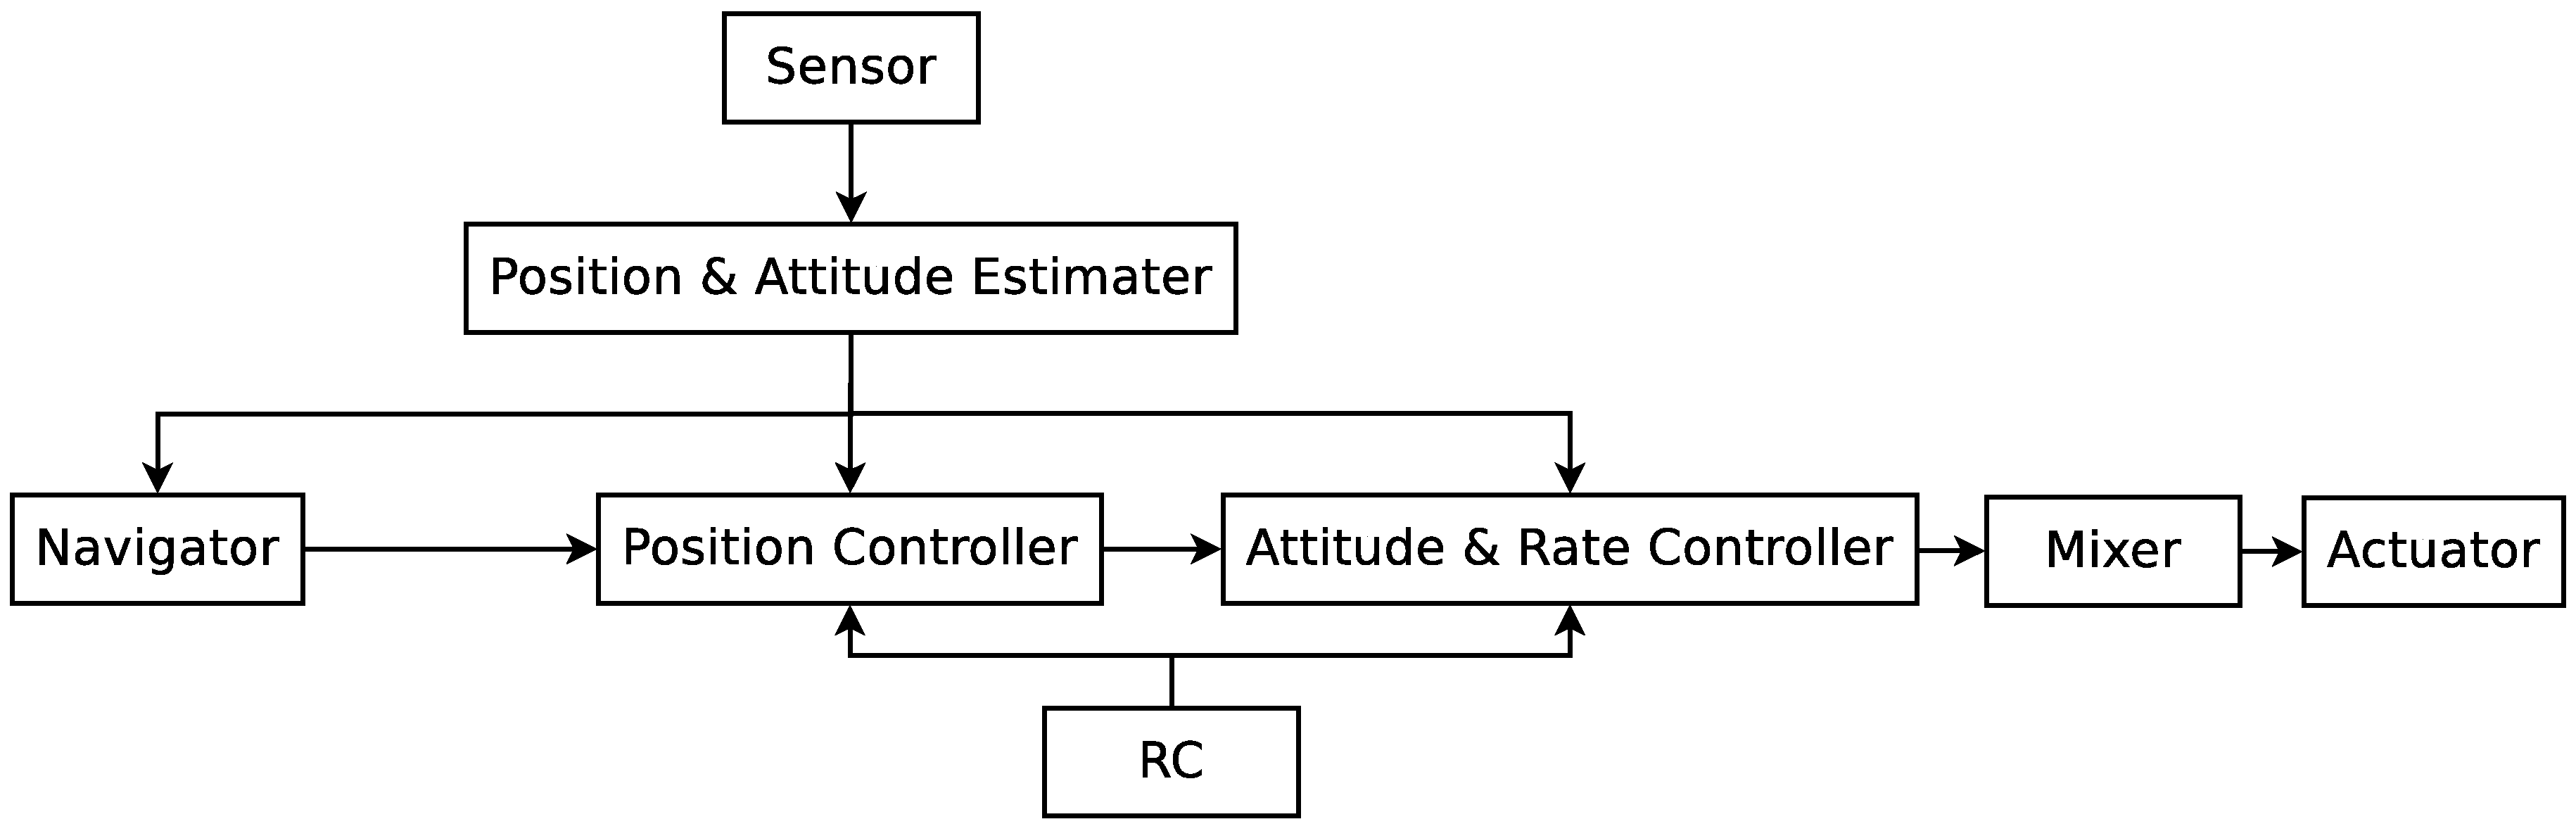
\includegraphics[width=0.9\linewidth]{flightStack.pdf}
	\caption{Overview of the PX4 flight stack}
	\label{fig:flightStack}
\end{figure}

PX4是Pixhawk开发的开源的飞控平台,能够
PX4 is an open source flight control platform that is supported by the Pixhawk flight control board, an independent open-hardware project for drones and other unmanned vehicles developed by Computer Vision and Geometry Laboratory at ETH Zurich.
Due to the clear structure of PX4 flight stack, shown in Fig.~\ref{fig:flightStack}. it is easy for developers to add their own flight mode on Pixhawk hardware board with PX4 software, or in the \jMAVSim{} tool that is a simulator for PX4-controlled unmanned aircraft.
We integrated the collision avoidance module we developed into the PX4 flight stack by adding it in the  position controller, the PX4 component responsible for the flight trajectory.


\subsection{Experiments Configuration}
\label{ssec:experimentsConfiguration}

In the experiments, since our Pixhawk drone has no sensors for detecting an intruder, we have created synthetic encounter situations where our own aircraft detects an intruder while performing a flight mission, so there may be a collision. 
The flight mission of our own aircraft is to reach the destination placed at 30 meters North of the initial position. 
The intruder aircraft starts from our destination and its goal is to reach our initial position.
When an encounter occurs, the intruder aircraft is designed to fly according to two predefined policies, introduced later in Sections~\ref{ssec:oppositeFlight} and~\ref{ssec:randomInterferingFlight}.
By following the sensor modeling given in Section~\ref{ssec:sensorModeling}, our own aircraft makes a detection every second, and the detection radius is set to 10 meters. 
That is, our own aircraft gets one observation per second about the presence and position of an intruder aircraft; 
it can be sensed when the distance between the two aircraft is below 10 meters. 
After getting the observation about the intruder aircraft, our own aircraft will react according to the two different collision avoidance methods introduced below.

\paragraph*{Simple rule-based collision avoidance scenario.}
In the simple rule-based collision avoidance scenario, our own aircraft reacts to observations as follows:
if $L$ or $R$ is observed (i.e., the intruder aircraft is in the detection range on the left or right of our aircraft), then bank to the opposite direction by $\frac{\pi}{6}$ and fly forward by $1$ meter;
otherwise $N$ is observed, so fly towards to destination.

\paragraph*{MCVI-based collision avoidance scenario.}
In the collision avoidance scenario using the MCVI synthesized policy, our own aircraft reacts to observations as follows:
as soon as an intruder aircraft is detected (observations $L$ and $R$), bank according to the policy as long as the intruder is detected or the graph terminal node is reached.
If the intruder aircraft is not detected or the policy graph terminal node is reached, fly towards the destination.
The banking angle and step length are the same as those of the simple rule-based method.
Note that after the controller stops to follow the policy, if the intruder aircraft is detected again, the controller restarts to follow the policy. 

\paragraph*{Experiments setting.}
Finally, we implemented the above two collision avoidance methods in the PX4 platform.
Supported by the \textsf{Software In the Loop} (SITL) simulation of the PX4 platform, we used \jMAVSim to  simulate our experiments. 
\jMAVSim{} supports the multirotor simulation and allows us to fly drones running PX4 in a synthetic world. 
To compare the effectiveness of two collision avoidance methods, we recorded the following measure data (with the meter as the length unit) to indicate the performance:
the number \emph{actNum} of banking performed to reach the destination,
the minimum distance \emph{minDis} between our own aircraft and the intruder aircraft,
the maximum deviation distance \emph{maxDvtDis} from the designed mission flight path, and
the increased flight distance \emph{incFltDis} from the original mission flight distance.




\subsection{Simulated Intruder's Opposite Flight Experiment}
\label{ssec:oppositeFlight}

\begin{figure}[t]
    \centering
	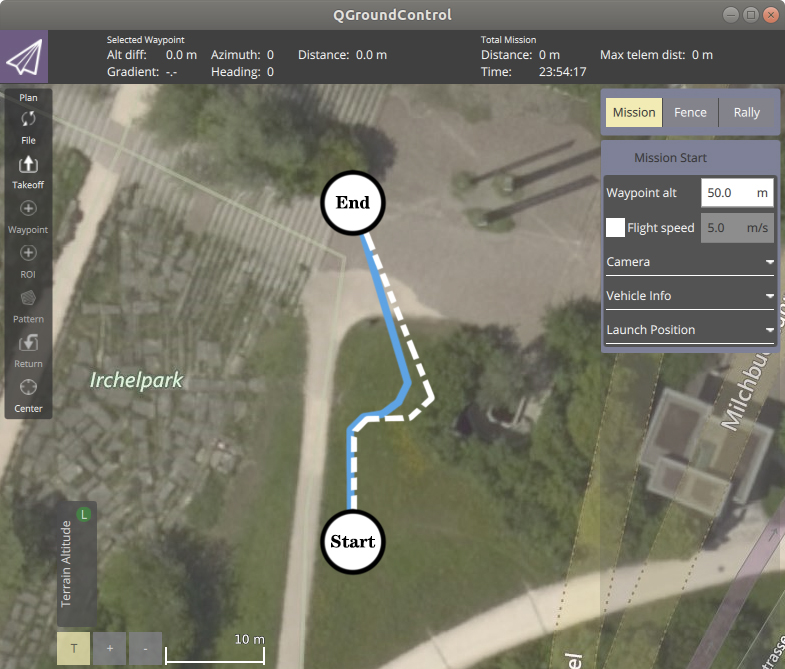
\includegraphics[width=0.95\linewidth]{oppositeFlightSimulation.jpg} 
	\caption{One flight simulation for the opposite flight experiment. Blue line: MCVI flight path; white line: simple flight path}
	\label{fig:oppositeFlightSimulation}
\end{figure}

\begin{table}[t]
	\caption{Opposite flight results; in bold, the best results}
	\label{tab:oppositeFlightResults}
	\centering
	\begin{tabular}{c|c|c}
		& rule-based & MCVI-based\\
		\hline 
		actNum & \textbf{4} & 5\\
		minDis & 2.51 & \textbf{2.95} \\
		maxDvtDis & 9.69 & \textbf{5.88} \\
		incFltDis & 14.83 & \textbf{9.67}\\
	\end{tabular}
\end{table}

In the first simulated experiment, we assume that the intruder aircraft starts from the destination of our own aircraft (viz. 30 meters North of the starting place of own aircraft) and flies straight towards the starting place of our own aircraft.
The flight paths of the mission while avoiding a collision are shown in Fig.~\ref{fig:oppositeFlightSimulation} and the average experimental results are summarized in Table~\ref{tab:oppositeFlightResults}.

Based on the \jMAVSim{} simulation, depicted in Fig.~\ref{fig:oppositeFlightSimulation}, we can see the flight path of own aircraft in the simulated map, where the blue solid line represents the flight path induced by the MCVI method while the white dashed line tracks the flight path given by the simple rule-based method. 
It can be intuitively seen from the figure that the MCVI method can reduce the useless avoidance distance of our own aircraft, and avoid the collision risk more effectively.

Table~\ref{tab:oppositeFlightResults} gives more details about the flight paths: 
we note that although the logic generated by MCVI based on the POMDP model takes 5 actions instead of 4 to reach the destination while avoiding the intruder aircraft, it does not results in an increase of the flight distance.
On the contrary, as shown in Fig.~\ref{fig:oppositeFlightSimulation} by the MCVI method's blue solid line being closer to the straight line between the terminal points than the simple method's white dashed line, the flight distance is increased by just 9.67 meters, about 5 meters less than the 14.83 meters of the simple method.
Furthermore, the MCVI-based approach increases the minimum distance (2.95 vs. 2.51 meters) from the intruder aircraft while deviating less (5.88 vs. 9.69 meters) from the optimal path without intruders than the simple method; 
this guarantees a higher safety level while decreasing the maximum deviation distance from the new flight path to the original mission flight path. 


\subsection{Simulated Intruder's Random Interfering Flight Experiment}
\label{ssec:randomInterferingFlight}

In the second simulated experiment, we assume that the intruder aircraft takes off from the midway between the start place and destination of our own aircraft (viz. 15 meters North of the starting place of our own aircraft). 
This time the intruder aircraft chooses randomly an action between bank-left, go-forward and bank-right, i.e., each one with probability $\frac{1}{3}$. 
Since the flight behavior of the intruder aircraft in this experiment is randomized, we repeated the simulation 50 times and then considered the average outcomes of the two scenarios against the same intruder's random choices, which can be reproduced by fixing the same random seed for the two scenarios. 

\begin{table}[t]
	\caption{Random interfering flight results; in bold, the best results}
	\label{tab:randomInterferingFlightAverageResults}
	\centering
	\begin{tabular}{c|cc|cc}
	& \multicolumn{2}{c|}{average value} & \multicolumn{2}{c}{median value}\\
	& rule-based & MCVI-based & rule-based & MCVI-based\\
	\hline
	actNum & \textbf{3.82} & 4.96 & \textbf{2.5} & 4 \\
	minDis & 5.54 & \textbf{6.06} & 5.88 & \textbf{6.04} \\
	maxDvtDis & 8.85 & \textbf{5.40} & 7.50 & \textbf{5.60} \\
	incFltDis & 9.14 & \textbf{7.10} & \textbf{6.67} & 6.87
	\end{tabular}
\end{table}
The statistics for this experiment are presented in Table~\ref{tab:randomInterferingFlightAverageResults};
as we can see, we have a behavior similar to the opposite flight experiment: 
although the logic generated by MCVI on the POMDP model banks on average one time more to avoid the intruder than the simple rule-based method, it is able to reduce the increased flight distance.
Furthermore, it increases the minimum distance between the two aircraft, which implies that the MCVI method gives a higher safety level when dealing with the random behavior of the intruder aircraft.
It is particularly noteworthy that when compared with the simple rule-based method, MCVI-based collision avoidance is able to save about $40\%$ of the maximum deviation distance between the actual flight path and the original mission flight path, which is a straight line between the designed takeoff and landing coordinates. 

We now give some more details about the safety level achieved by the two collision avoidance scenarios introduced in Section~\ref{ssec:experimentsConfiguration}.
Out of the 50 simulations for each of the two scenarios, 
both scenarios ensure that there is no collision since in none of the simulations the minimum distance was below $2$ meters, the value we set for NMAC;
the minimum distance has been at least $2.5$ meters.
There have been few simulations where the distance was about 3 meters and the majority above 4 meters, with the MCVI-based scenario usually keeping a larger distance.
This is reflected also by the average \emph{minDis} values reported in Table~\ref{tab:randomInterferingFlightAverageResults}, where the rule-based \emph{minDis} value is lower than the one for MCVI, which means that the former control policy got closer to the intruder than the latter one.

From these experiments, we obtain that the MCVI-based collision avoidance controller provides a better safety level, since it keeps a larger distance between our aircraft and the intruder than the rule-based controller.
This comes at the cost of banking the aircraft few more times, which still allows for reducing the increased flown distance.
The flown distance is also an aspect to be considered for drones and other unmanned aircraft, since the increased flight distance reduces the actual operative range of the aircraft, given the limited amount of energy stored in the batteries that can be used to power the aircraft.

While the experiments give a good indication about the safety level provided by the MCVI-based collision avoidance controller, there is no guarantee that it always avoids collisions.
We leave the formal analysis of its safety as future work.


\subsection{Actual Pixhawk Drone Flight Experiment}
\label{ssec:realDrone}

In the third experiment, we have taken the PX4 MCVI-based collision avoidance module we developed and uploaded it on a real Pixhawk drone we assembled ourselves. %, shown in Fig.~\ref{fig:RealDrone}. 
The flight mission is the same as for the previous experiments. 
The Pixhawk drone communicates to its ground station several data about the position and flight attitude.
Since the Pixhawk drone has no sensors for detecting intruders, we used the ground station to inject in the drone's PX4 control system the synthetic intruder from the opposite flight experiment presented in Section~\ref{ssec:oppositeFlight}.
We show in Fig.~\ref{fig:realFlightPath} the actual flight path flown by our drone as registered by the ground control station and superimposed on the map.

\begin{figure}[t]
	\centering 
	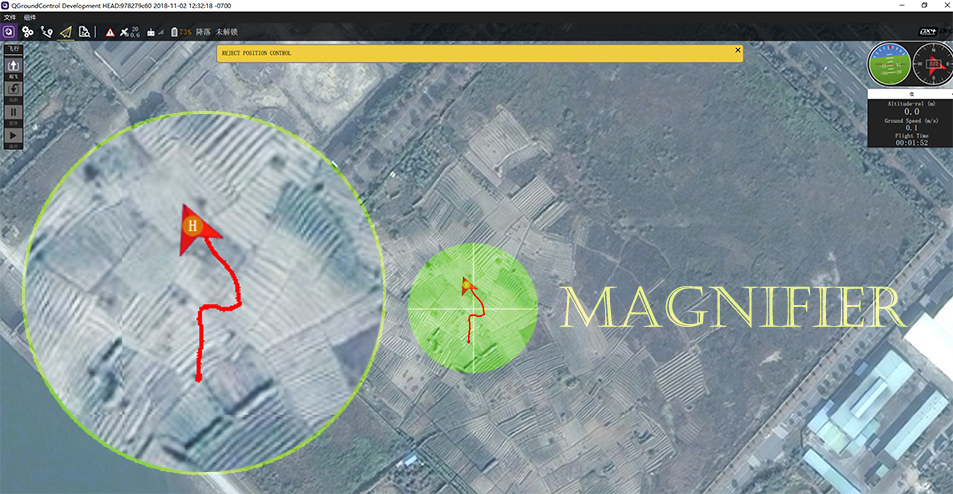
\includegraphics[width=1\linewidth]{realFlightPath.jpg}
	\caption{The actual Pixhawk drone flight path registered by the ground control station}
	\label{fig:realFlightPath}
\end{figure}

As we can see, the MCVI-based collision avoidance module works well not only in a synthetic environment, but also in the real world.
This suggests that the policy synthesis for specifically crafted POMDPs can improve the safety of unmanned aircraft equipped with a collision avoidance module basing its decisions on the synthesized policy.



\section{Conclusion}
\label{sec:conclusion}

We have constructed a collision avoidance system working with limited information, which also tried to save flying resources by means of reducing the change of the original flight path.
Our approach used a POMDP to model the collision avoidance system with only the destination information of our own aircraft and rough direction information of the intruder and then generated the collision resolution logic that maximizes the expected sum of rewards of selected actions.
We have implemented the collision avoidance module and embedded it into the PX4 flight control platform that can control real unmanned aircraft systems.
The effectiveness of our system is witnessed by the experimental evaluation in both a simulated environment and a real world scenario using a Pixhawk drone.

As future work, we consider to study the scalability of the MCVI approach to more detailed flight scenarios, such as the ones with the 3D environment, different aircraft speeds, more accurate observations given by better sensors, and so on.
Also, we plan to apply machine learning algorithms to improve the efficiency of the algorithm for searching an optimal policy.
Moreover, we also consider the use of rigorous methods, such as model checking, to ensure the correctness of the collision avoidance system.


\end{document}